\chapter{Arhitektura i dizajn sustava}
		\textit{ Izbor odgovarajuće arhitekture programske poruke jedan je od najbitnijih koraka u oblikovanju sustava jer ona predstavlja poveznicu između zahtjeva na sustav i same implementacije sustava. Dobra arhitektura povlači dobru fleksibilnost sustava, jednostavnu mogućnost nadogradnje i jeftino održavanje.}
		
		\textit{ S obzirom da je zadatak ovog projekta napraviti aplikaciju za šahovski klub, logičan izbor je web aplikacija. Primarni razlog je to što web aplikacija ne ovisi o platformi, već radi na svakom sustavu koji ima web preglednik što znatno smanjuje vrijeme i troškove potrebne za razvoj za više platformi}
		
		\textit{ Radni okvir koji smo odabrali za arhitekturu je Django (pisan u i za jezik Python). S njime smo arhitekturu sustava odlučili temeljiti na MVT (Model-View-Template) konceptu kojeg on nativno podržava. Jedina bitna razlika između njega i poznatog MVC (Model-View-Controller) koncepta je to što u Django sam po sebi sređuje "controller" dio (programski kod koji kontrolira interakciju između modela i viewa) i daje nam na raspolaganje Template.}
		
		\textit{ Dakle aplikacija se sastoji od 3 dijela: }
		\begin{itemize}
			\item 	\textit{Model - Sređuje apstrakciju podataka, služi kao sučelje za podatke spremljene u bazu i dopušta upravljanje njima bez prevelikog razumijevanja kompleksnosti same baze }
			\item 	\textit{View - funkcionalnosti slične controlleru u MVC konceptu. Sređuje svu logiku koja se treba prikazati na templateu i služi kao "most" između modela i templatea}
			\item 	\textit{Template - funkcionalnosti slične Viewu u MVC konceptu. Služi kao sloj prikaza sadržaja i zadužen je za to kako i što će biti prikazano korisniku. Specifično za Django, Template je vrsta HTML datoteke koja može koristiti Django Template Language (DTL) što nam znatno olakšava komunikaciju između frontenda i backenda aplikacije.}		
		\end{itemize}
		

				
		\section{Baza podataka}
			
			\textbf{\textit{dio 1. revizije}}\\
			
		\textit{Potrebno je opisati koju vrstu i implementaciju baze podataka ste odabrali, glavne komponente od kojih se sastoji i slično.}
		
			\subsection{Opis tablica}
			

				\textit{Svaku tablicu je potrebno opisati po zadanom predlošku. Lijevo se nalazi točno ime varijable u bazi podataka, u sredini se nalazi tip podataka, a desno se nalazi opis varijable. Svjetlozelenom bojom označite primarni ključ. Svjetlo plavom označite strani ključ}
				
				\begin{longtabu} to \textwidth {|X[6, l]|X[6, l]|X[20, l]|}
					
					\hline \multicolumn{3}{|c|}{\textbf{korisnik - ime tablice}}	 \\[3pt] \hline
					\endfirsthead
					
					\hline \multicolumn{3}{|c|}{\textbf{korisnik - ime tablice}}	 \\[3pt] \hline
					\endhead
					
					\hline 
					\endlastfoot
					
					\cellcolor{LightGreen}IDKorisnik & INT	&  	Lorem ipsum dolor sit amet, consectetur adipiscing elit, sed do eiusmod tempor incididunt ut labore et dolore magna aliqua. Ut enim ad minim veniam 	\\ \hline
					korisnickoIme	& VARCHAR &   	\\ \hline 
					email & VARCHAR &   \\ \hline 
					ime & VARCHAR	&  		\\ \hline 
					\cellcolor{LightBlue} primjer	& VARCHAR &   	\\ \hline 
					
					
				\end{longtabu}
				
				\begin{longtabu} to \textwidth {|X[6, l]|X[6, l]|X[20, l]|}
					
					\hline \multicolumn{3}{|c|}{\textbf{taktika}}	 \\[3pt] \hline
					\endfirsthead
					
					\hline \multicolumn{3}{|c|}{\textbf{taktika}}	 \\[3pt] \hline
					\endhead
					
					\hline 
					\endlastfoot
					
					\cellcolor{LightGreen}idTaktika & INT	   &  identfikacijski broj taktike	\\ \hline
					createdAt	& TIMESTAMP &   vrijeme stvaranja taktike, služi za kronološko sortiranje taktika	\\ \hline 
					\cellcolor{LightBlue}idUser & INT & identifikator trenera ili admina koji je stvorio taktiku  \\ \hline 
					initConfig & VARCHAR (100)	&  string koji opisuje inicijalno stanje šahovske ploče	\\ \hline 
					movesWhite & VARCHAR (3000) & string koji opisuje poteze bijelih figurica \\ \hline
					movesBlack & VARCHAR (3000) & string koji opisuje poteze crnih figurica \\ \hline
					tezina & DECIMAL & težina taktike, koristi se u računanju bodova, u rasponu od 1 do 3 \\ \hline
					brojGlasova & INT & broj korisnika koji su glasali za neku težinu taktike \\ \hline

				\end{longtabu}

				\begin{longtabu} to \textwidth {|X[6, l]|X[6, l]|X[20, l]|}
					
					\hline \multicolumn{3}{|c|}{\textbf{rjesenjeTaktika}}	 \\[3pt] \hline
					\endfirsthead
					
					\hline \multicolumn{3}{|c|}{\textbf{rjesenjeTaktika}}	 \\[3pt] \hline
					\endhead
					
					\hline 
					\endlastfoot
					
					\cellcolor{LightGreen}idTaktika & INT	   &  identfikacijski broj taktike koja je rješena, foreign key	\\ \hline
					\cellcolor{LightGreen}idUser & INT & identifikator člana koji je riješio taktiku, foreign key  \\ \hline 
					vrijeme & DECIMAL & vrijeme rješavanja taktike u minutama \\ \hline
					
				\end{longtabu}
				
				\begin{longtabu} to \textwidth {|X[6, l]|X[6, l]|X[20, l]|}
					
					\hline \multicolumn{3}{|c|}{\textbf{dojavaPogreske}}	 \\[3pt] \hline
					\endfirsthead
					
					\hline \multicolumn{3}{|c|}{\textbf{dojavaPogreske}}	 \\[3pt] \hline
					\endhead
					
					\hline 
					\endlastfoot
					
					\cellcolor{LightGreen}idDojava & INT	   &  identfikacijski broj dojave o pogrešci	\\ \hline
					\cellcolor{LightBlue}idTaktika & INT	   &  identfikacijski broj prijavljene taktike	\\ \hline
					\cellcolor{LightBlue}idUserDojavio & INT & identifikator člana koji je dojavio pogrešku na taktiku  \\ \hline 
					\cellcolor{LightBlue}idUserRevidira & INT & identifikator trenera koji revidira dojavu  \\ \hline 
					prihvacena & BOOLEAN	&  je li dojava prihvacena ili odbacena, NULL znači da čeka na revidiranje	\\ \hline 
					predlozeniTijek & VARCHAR (6000) & string koji opisuje poteze koje je predložio član koji je dojavio pogrešku \\ \hline
					opisPoteza & TEXT & opis poteza koje je član unio \\ \hline
					
				\end{longtabu}
				
				\begin{longtabu} to \textwidth {|X[6, l]|X[6, l]|X[20, l]|}
					
					\hline \multicolumn{3}{|c|}{\textbf{view - rangLista}}	 \\[3pt] \hline
					\endfirsthead
					
					\hline \multicolumn{3}{|c|}{\textbf{view - rangLista}}	 \\[3pt] \hline
					\endhead
					
					\hline 
					\endlastfoot
					
					\cellcolor{LightGreen}idUser & INT	   &  identfikacijski broj člana	\\ \hline
					username & VARCHAR	   &  korisničko ime člana	\\ \hline
					bodovi & INT & broj bodova koje je član sveukupno osvojio \\ \hline 
					
				\end{longtabu}
			
				\begin{longtabu} to \textwidth {|X[6, l]|X[8, l]|X[20, l]|}
					
					\hline \multicolumn{3}{|c|}{\textbf{Korisnik}}	 \\[3pt] \hline
					\endfirsthead
					
					\hline \multicolumn{3}{|c|}{\textbf{Korisnik}}	 \\[3pt] \hline
					\endhead
					
					\hline 
					\endlastfoot
					
					\cellcolor{LightGreen} idUser & INT &  identfikacijski broj člana \\ \hline
					\cellcolor{LightBlue} idGrupa & INT & identifikacijski broj grupe \\ \hline
					username & VARCHAR (20) &  korisničko ime člana \\ \hline 
					password & VARCHAR (20) & lozinka člana \\ \hline 
					email & VARCHAR (20) & mail adresa člana \\ \hline
					ime & VARCHAR (20) & ime člana \\ \hline
					prezime & VARCHAR (20) & prezime člana \\ \hline
					
				\end{longtabu}
			
				\begin{longtabu} to \textwidth {|X[6, l]|X[8, l]|X[20, l]|}
				
					\hline \multicolumn{3}{|c|}{\textbf{Grupa}}	 \\[3pt] \hline
					\endfirsthead
					
					\hline \multicolumn{3}{|c|}{\textbf{Grupa}}	 \\[3pt] \hline
					\endhead
					
					\hline 
					\endlastfoot
					
					\cellcolor{LightGreen} idGrupa & INT & identifikacijski broj grupe \\ \hline
					imeGrupe & VARCHAR (20) &  ime grupe \\ \hline
				
				\end{longtabu}
				
				\begin{longtabu} to \textwidth {|X[10, l]|X[8, l]|X[20, l]|}
				
					\hline \multicolumn{3}{|c|}{\textbf{Novost}}	 \\[3pt] \hline
					\endfirsthead
					
					\hline \multicolumn{3}{|c|}{\textbf{Novost}}	 \\[3pt] \hline
					\endhead
					
					\hline 
					\endlastfoot
					
					\cellcolor{LightGreen} idUser & INT & identifikacijski broj autora \\ \hline
					\cellcolor{LightGreen} vrijemeObjavljivanja & DATETIME & vrijeme i datum objavljivanja \\ \hline
					naslov & VARCHAR (50) & naslov novosti\\ \hline
					tekst & TEXT & tekst novosti\\ \hline
				
				\end{longtabu}

				\begin{longtabu} to \textwidth {|X[10, l]|X[8, l]|X[20, l]|}
				
					\hline \multicolumn{3}{|c|}{\textbf{Trening}}	 \\[3pt] \hline
					\endfirsthead
					
					\hline \multicolumn{3}{|c|}{\textbf{Trening}}	 \\[3pt] \hline
					\endhead
					
					\hline 
					\endlastfoot
					
					\cellcolor{LightGreen} idTreninga & INT & identifikacijski broj treninga\\ \hline
					\cellcolor{LightBlue} idOrganizatora & INT & identifikacijski broj organizatora treninga \\ \hline
					vrijemePocetka & DATETIME & vrijeme i datum početka treninga\\ \hline
					vrijemeZavrsetka & DATETIME & vrijeme i datum završetka treninga\\ \hline
					opisTreninga & TEXT & opisan sadržaj treninga\\ \hline
				
				\end{longtabu}
				

				\begin{longtabu} to \textwidth {|X[10, l]|X[8, l]|X[20, l]|}
				
					\hline \multicolumn{3}{|c|}{\textbf{Turnir}}	 \\[3pt] \hline
					\endfirsthead
					
					\hline \multicolumn{3}{|c|}{\textbf{Turnir}}	 \\[3pt] \hline
					\endhead
					
					\hline 
					\endlastfoot
					
					\cellcolor{LightGreen} idTurnira & INT & identifikacijski broj turnira\\ \hline
					formatTurnira & TEXT & opisan format turnira \\ \hline
					vrijemePocetka & DATETIME & vrijeme i datum početka turnira\\ \hline
					vrijemeZavrsetka & DATETIME & vrijeme i datum završetka turnira\\ \hline
					brojSudionika & INT & maksimalan broj sudionika na turniru\\ \hline
				
				\end{longtabu}

				\begin{longtabu} to \textwidth {|X[10, l]|X[8, l]|X[20, l]|}
				
					\hline \multicolumn{3}{|c|}{\textbf{PrijavaTrening}}	 \\[3pt] \hline
					\endfirsthead
					
					\hline \multicolumn{3}{|c|}{\textbf{PrijavaTrening}}	 \\[3pt] \hline
					\endhead
					
					\hline 
					\endlastfoot
					
					\cellcolor{LightBlue} idClana & INT & identifikacijski broj člana\\ \hline
					\cellcolor{LightBlue} idTreninga & INT & identifikacijski broj treninga \\ \hline
				
				\end{longtabu}

				\begin{longtabu} to \textwidth {|X[10, l]|X[8, l]|X[20, l]|}
				
					\hline \multicolumn{3}{|c|}{\textbf{PrijavaTurnir}}	 \\[3pt] \hline
					\endfirsthead
					
					\hline \multicolumn{3}{|c|}{\textbf{PrijavaTurnir}}	 \\[3pt] \hline
					\endhead
					
					\hline 
					\endlastfoot
					
					\cellcolor{LightBlue} idClana & INT & identifikacijski broj člana\\ \hline
					\cellcolor{LightBlue} idTurnira & INT & identifikacijski broj turnira \\ \hline
				
				\end{longtabu}

				\begin{longtabu} to \textwidth {|X[10, l]|X[8, l]|X[20, l]|}
				
					\hline \multicolumn{3}{|c|}{\textbf{Transakcija}}	 \\[3pt] \hline
					\endfirsthead
					
					\hline \multicolumn{3}{|c|}{\textbf{Transakcija}}	 \\[3pt] \hline
					\endhead
					
					\hline 
					\endlastfoot
					
					\cellcolor{LightGreen} idTransakcije & INT & identifikacijski broj transakcije\\ \hline
					\cellcolor{LightBlue} idClana & INT & identifikacijski broj člana\\ \hline
					datumTransakcije & DATETIME & vrijeme i datum izvršavanja transakcije\\ \hline
					iznosUplate & DECIMAL & uplaćen iznos\\ \hline

				\end{longtabu}

				
			
			\subsection{Dijagram baze podataka}
			
			\begin{figure}[H]
					\centerfloat
        					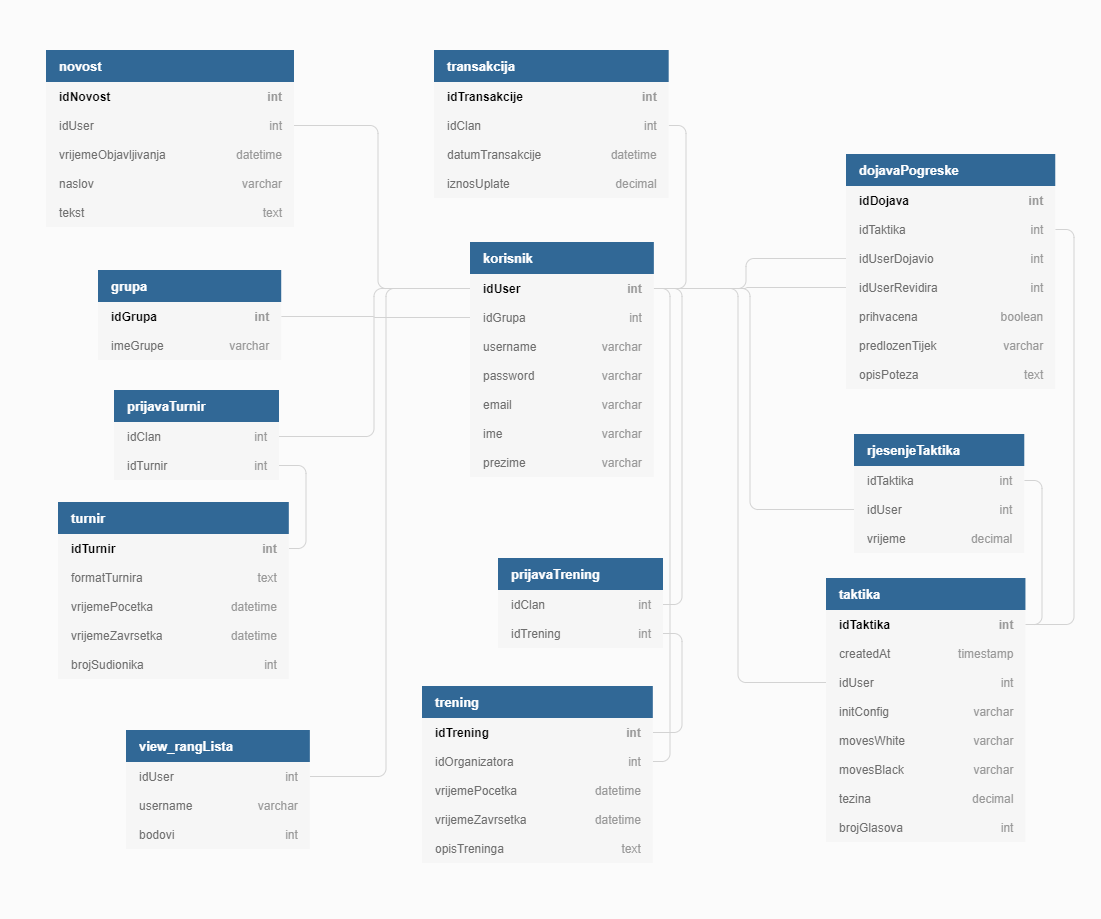
\includegraphics[scale=0.60]{dijagrami/dijagramBaze.png} %veličina slike u odnosu na originalnu datoteku i pozicija slike
        					\caption{E-R dijagram baze podataka}
        					\label{fig:DBdiagram}
				\end{figure}
			
			\eject
			
			
		\section{Dijagram razreda}
		
			\textit{Potrebno je priložiti dijagram razreda s pripadajućim opisom. Zbog preglednosti je moguće dijagram razlomiti na više njih, ali moraju biti grupirani prema sličnim razinama apstrakcije i srodnim funkcionalnostima.}\\
			
			\textbf{\textit{dio 1. revizije}}\\
			
			\textit{Prilikom prve predaje projekta, potrebno je priložiti potpuno razrađen dijagram razreda vezan uz \textbf{generičku funkcionalnost} sustava. Ostale funkcionalnosti trebaju biti idejno razrađene u dijagramu sa sljedećim komponentama: nazivi razreda, nazivi metoda i vrste pristupa metodama (npr. javni, zaštićeni), nazivi atributa razreda, veze i odnosi između razreda.}\\
			
			\textbf{\textit{dio 2. revizije}}\\			
			
			\textit{Prilikom druge predaje projekta dijagram razreda i opisi moraju odgovarati stvarnom stanju implementacije}
			
			
			
			\eject
		
		\section{Dijagram stanja}
			
			
			\textbf{\textit{dio 2. revizije}}\\
			
			\textit{Potrebno je priložiti dijagram stanja i opisati ga. Dovoljan je jedan dijagram stanja koji prikazuje \textbf{značajan dio funkcionalnosti} sustava. Na primjer, stanja korisničkog sučelja i tijek korištenja neke ključne funkcionalnosti jesu značajan dio sustava, a registracija i prijava nisu. }
			
			
			\eject 
		
		\section{Dijagram aktivnosti}
			
			\textbf{\textit{dio 2. revizije}}\\
			
			 \textit{Potrebno je priložiti dijagram aktivnosti s pripadajućim opisom. Dijagram aktivnosti treba prikazivati značajan dio sustava.}
			
			\eject
		\section{Dijagram komponenti}
		
			\textbf{\textit{dio 2. revizije}}\\
		
			 \textit{Potrebno je priložiti dijagram komponenti s pripadajućim opisom. Dijagram komponenti treba prikazivati strukturu cijele aplikacije.}